\chapter{Structures de données classiques}
\minitoc
\section{\texttt{Pile}}
\lstinputlisting[language=C, caption=\texttt{Pile} sans protection du type -- Header]{content/code/pile.h}
	\subsection{Statique}
	\subsubsection{Sans protection du type}
\begin{itemize}
	\item Utilisation d'un tableau
	\item Utilisation d'un entier donnant le nombre d'éléments rangés dans la pile
\end{itemize}
\lstinputlisting[language=C, caption=\texttt{Pile} statique sans protection du type -- Implémentation]{content/code/pileStatique.c}

Amélioration de la \texttt{Pile}.
\begin{enumerate}
	\item Implémenter la fonction permettant de remplacer toute les occurrences de l'élément x par l'élément y dans la pile.
	\item Implémenter la fonction d'affichage de la Pile.
\end{enumerate}
\begin{description}
	\item[Rajouter dans le champ des opérations] \texttt{remplacerOccurence} Pile $\times$ Element $\times$ Element $\rightarrow$ Pile
	\item[Préconditions] rien
	\item[Axiones]
\end{description}

\begin{lstlisting}[language=C]
remplacerOccurence(creer(), x, y) = creer();
remplacerOccurence(empiler(p, x), x1, x2) = 
		p1 $\wedge$ $\forall z$ (appartient(p1, z) $\rightarrow$ (z $\neq$ x1) (empiler(p, x), z') $\wedge$ z' = x1))
\end{lstlisting}
\lstinputlisting[language=C, caption=\texttt{Pile} statique -- Ajout de \texttt{remplacerOccurence}]{content/code/pileStatique-2.c}
\subsubsection{Avec protection du type}
\lstinputlisting[language=C, caption=\texttt{Pile} statique avec protection du type -- Implémentation]{content/code/pileStatique-3.c}
\subsection{\texttt{Dynamique}}
Une pile dynamique peut être implémentée de différentes façons, la liste simplement chaînée et la liste doublement chaînée.
\begin{figure}[H]
\centering
\includegraphics[width=8cm]{content/schemas/pile.eps}
\caption{Pile avec une liste simplement chainée}
\end{figure}

\begin{figure}[H]
\centering
\includegraphics[width=16cm]{content/schemas/pileDoubleChaine.eps}
\caption{Pile avec une liste doublement chainée}
\end{figure}

Nous avons choisi de l'implémenter avec une liste simple chaînée, le double chaînage n'étant pas utile pour ce que nous souhaitons faire.
\lstinputlisting[language=C, caption=\texttt{Pile} dynamique -- Implémentation]{content/code/pileDynamique.c}

\section{\texttt{File}}
\begin{description}
	\item[Sorte] File
	\item[Utilise] Element, booleen
	\item[Constructeurs]~
		\begin{description}
			\item[\texttt{creer}] $\rightarrow$ File% CONSTRUCTEURS
			\item[\texttt{enfiler}] \texttt{File} $\times$ Element $\rightarrow$ File
		\end{description}
	\item[Projecteurs] 
		\begin{description}
			\item[\texttt{estVide}] file $\rightarrow$ Booleen
			\item[\texttt{appartient}] file $\times$ Element $\rightarrow$ Booleen
			\item[\texttt{defiler}] file $\rightarrow$ file
			\item[\texttt{premier}] file $\rightarrow$ Element
			\item[\texttt{dernier}] file $\rightarrow$ Element
		\end{description}
	\item[Précondition]~
		\begin{description}
			\item[\texttt{premier}] premier(f) $\Leftrightarrow$ $\neg$estVide(f) 
			\item[\texttt{dernier}] dernier(f) $\Leftrightarrow$ $\neg$estVide(f) 
		\end{description}
	\item[Axiones]~
		\begin{lstlisting}[language=C, numbers=none,caption=\texttt{File} -- Axiones]
estVide(creer()) = true;
estVide(enfiler(f,x)) = false;
appartient(creer(), x) = false;
appartient(enfiler(f,x),y) = (x = y) $\vee$ appartient(f,y)
defiler(creer()) = creer()
defiler(enfiler(f,x) = creer() si estVide(f)
					 = enfiler(defiler(f), x) sinon
premier(enfiler(f,x)) = premier(f) si !estVide
					  = x sinon
dernier(enfiler(f,x)) = x
\end{lstlisting}
\end{description}
	\lstinputlisting[language=C, caption=\texttt{File} -- Headers]{content/code/file.h}
	\subsection{Statique}
\lstinputlisting[language=C, caption=\texttt{File} statique -- Implémentation]{content/code/fileStatique.c}
	\subsection{Dynamique}
	De la même manière que la pile, en dynamique la \texttt{File} peut être implémentée avec une liste simplement chaînée ou une liste doublement chaînée.
\begin{figure}[H]
\centering
\includegraphics[width=10cm]{content/schemas/file.eps}
\caption{File avec une liste simplement chainée}
\end{figure}

\begin{figure}[H]
\centering
\includegraphics[width=15cm]{content/schemas/fileDoubleChaine.eps}
\caption{File avec une liste doublement chainée}
\end{figure}
Nous avons choisis la liste simplement chaînée.
\lstinputlisting[language=C, caption=\texttt{File} dynamique -- Implémentation]{content/code/fileDynamique.c}

\subsubsection{Application de la \texttt{File} à la fusion de voies routières}
\paragraph{Amélioration de la \texttt{File} en dynamique} Ecrire dans le module \texttt{File} (en dynamique) les deux fonctions suivantes : 
\begin{itemize}
	\item \texttt{concat}: \texttt{File} $\times$ \texttt{File} $\rightarrow$ \texttt{File}
	\item \texttt{mixe}: \texttt{File} $\times$ \texttt{File} $\rightarrow$ \texttt{File}
\end{itemize} ~

\lstinputlisting[language=C, caption=\texttt{File} dynamique -- Ajout \texttt{concat} et \texttt{mixe}]{content/code/fileDynamique-2.c}
\paragraph{Écrire l'application} ~
\lstinputlisting[language=C, caption=\texttt{File} -- Application de fusion de voies routières]{content/code/fileAppli.c}
\section{\texttt{File} avec priorité}
Ce sont des files dans lesquelles on place chaque élément au <<bon endroit>> (en remplaçant les priorités), en l'occurrence, les éléments doivent être triés par
\texttt{Element}.

On va considérer qu'il existe dans le module \texttt{Element}, une fonction qui permet de comparer deux éléments entre eux.
\begin{lstlisting}[language=C, numbers=none,caption=Element -- Prototype \texttt{comparer}]
/*
 * Renvoie   0 si e1 et e2 sont de même priorité
 *			-1 si e1 est moins prioritaire que e2
 *           1 si e1 est plus prioritaire que e2
 */
int compare(elem e1, elem e2);
\end{lstlisting}
\attention{Le main de la fonction pourrait changer suivant les éléments}
Réécrire \texttt{enfiler} en utilisant un pointeur de fonction pour accéder à la fonction de comparaison.
\section{\texttt{Liste} avec priorité}
Nous allons utiliser une liste doublement chaînée.
\begin{figure}[H]
	\centering
\includegraphics[width=12cm]{content/schemas/fileDoubleChaine.eps}
	\caption{Liste doublement chaînée}
\end{figure}

\begin{enumerate}
	\item Proposer un type C pour la liste doublement chainée
	\item \'Ecrire les méthodes suivantes:  \\
\begin{lstlisting}[language=C, numbers=none]
LDC creer();
LDC ajouter(LDC, Elem);
void affichageCroisant(LDC);
void afficheDecroissant(LDC);
LDC supprimer(LDC, Elem);
/* Application de la fonction à chaqcun des éléments de la LDC et renvoie
 * la LDC des résultats 
 */
LDC map(fonction, LDC) 
\end{lstlisting}
\end{enumerate}
\lstinputlisting[language=C, caption=\texttt{Liste} doublement chainée -- Header]{content/code/listeDoublementChaine.h}
\lstinputlisting[language=C, caption=\texttt{Liste} doublement chainée -- Implémentation]{content/code/listeDoublementChaine.c}

